\documentclass[fleqn, a4paper. 12pt]{ltjsarticle} 
% following is the compile command (以下のコマンドでコンパイル可能)
% $ lualatex guidance.tex 
% you need to install texlive to execute the above.(texlive を入れる必要がある.)
\usepackage{amsmath,txfonts}
\usepackage{amssymb}
\usepackage{url}
\usepackage{subcaption}
\usepackage[margin=31mm]{geometry}
\usepackage{graphicx}
\usepackage{listings}


\begin{document}
\begin{titlepage}
      \begin{center}
      {
      \Huge 2023年度\\言語処理 課題}
      
      \vspace{4cm}
             {\Huge 言語処理\\
               実験レポート\\}
             \vspace{4cm}
                    {\large 提出日:2024年2月7日(水)\\}
                    
                    {\large 学修番号:22140003\\氏名:佐倉仙汰郎}
    \end{center}  
  \end{titlepage}

  \section{課題1}
  \begin{figure}[h]
    \centering
    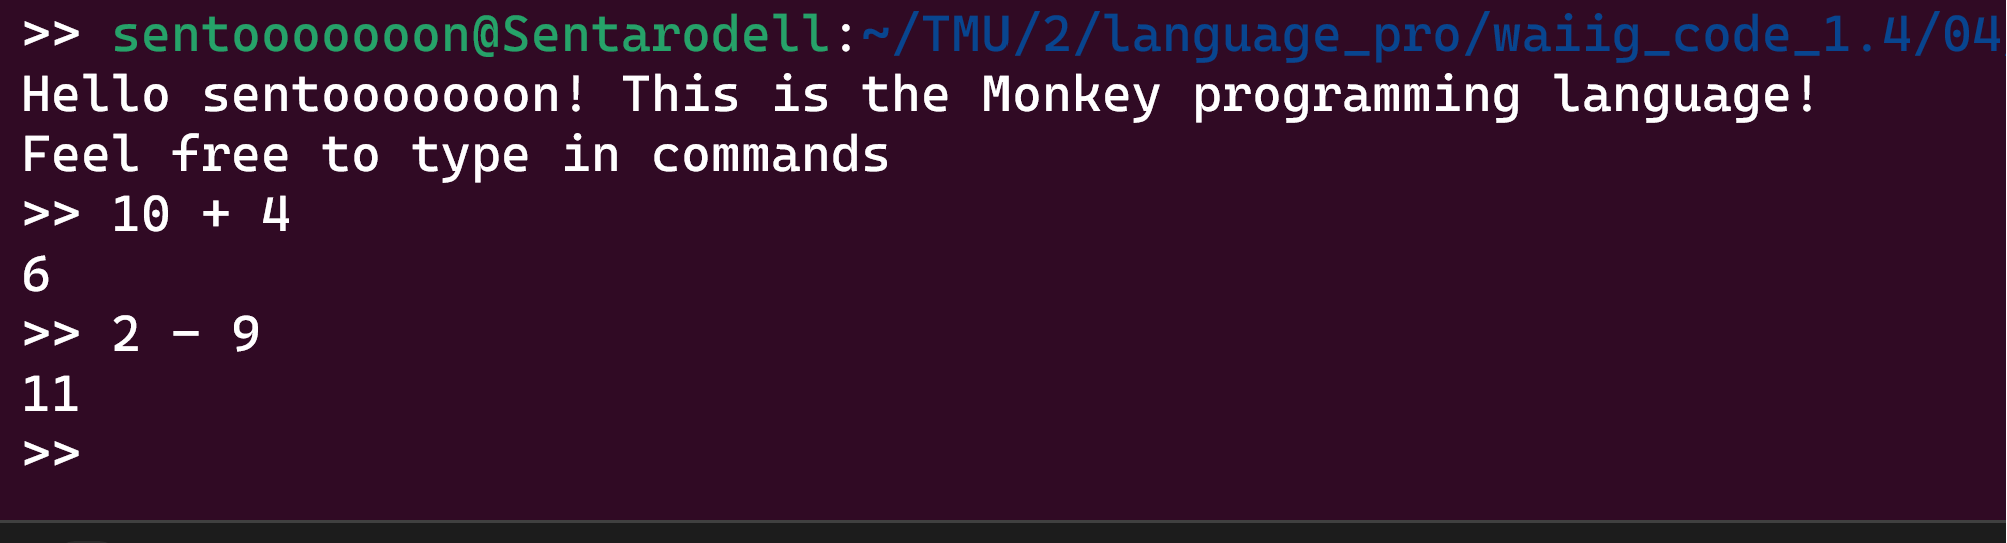
\includegraphics[width=0.5\linewidth]{images/1_a.png}
    \label{fig:example}
\end{figure}
\begin{figure}[h]
    \centering
    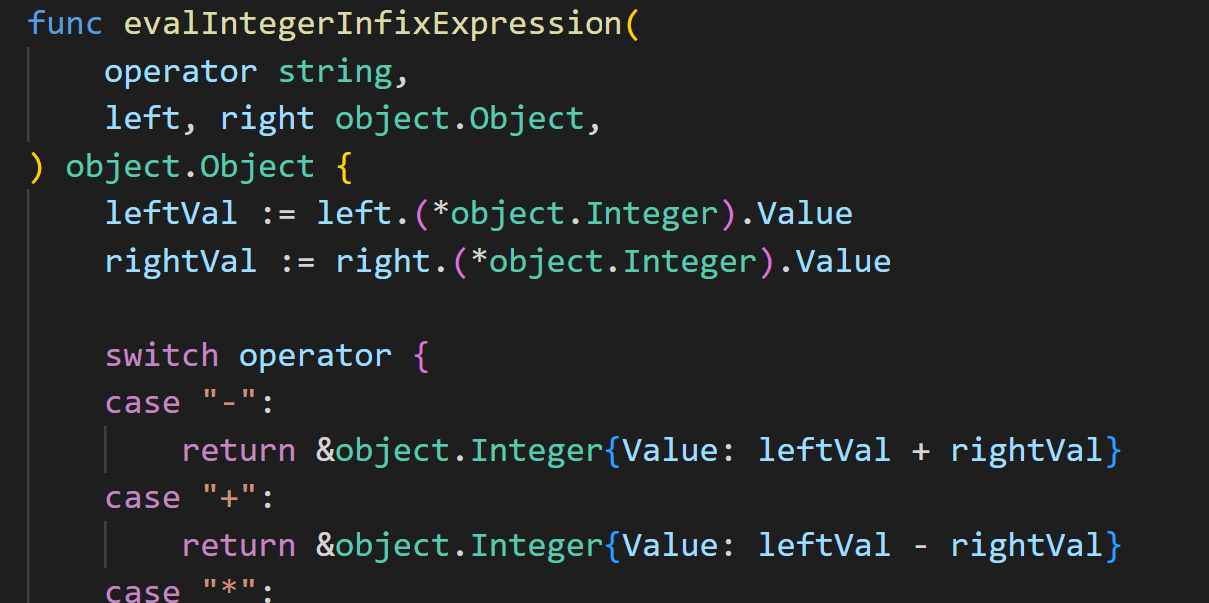
\includegraphics[width=0.5\linewidth]{images/1_b.png}
    \label{fig:example}
\end{figure}
\section{課題2}
\begin{figure}[h]
    \centering
    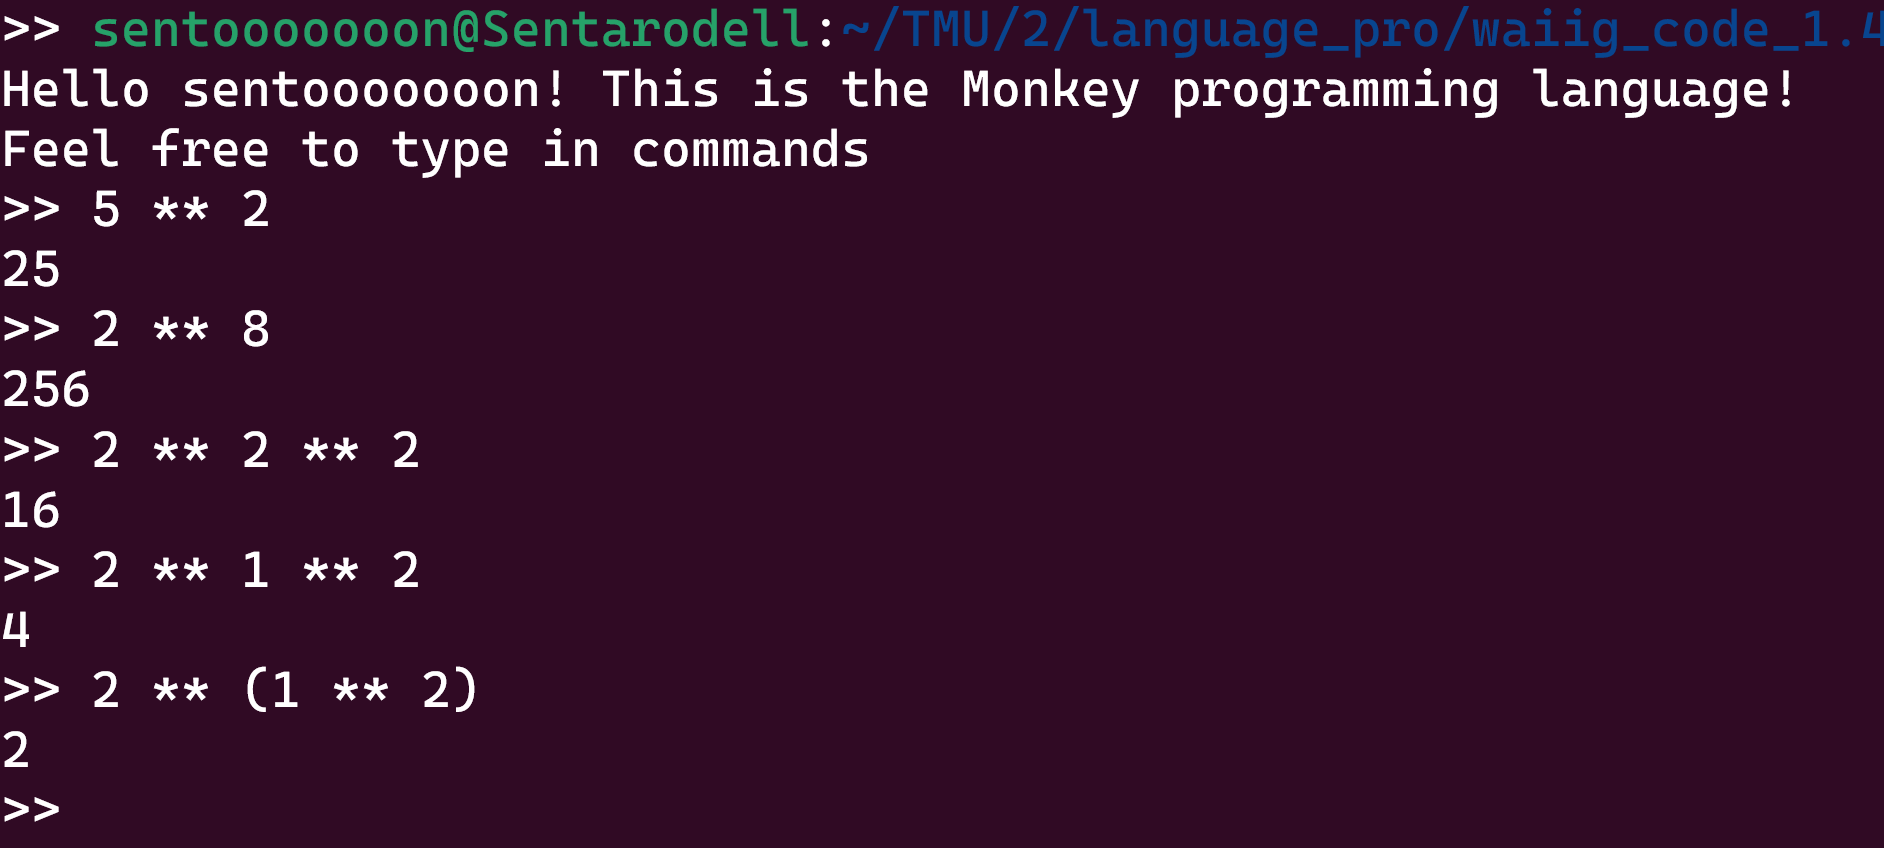
\includegraphics[width=0.5\linewidth]{images/2_result.png}
    \label{fig:example}
\end{figure}
\begin{figure}[h]
    \centering
    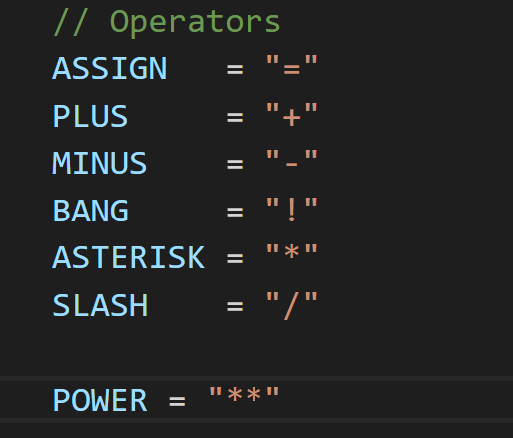
\includegraphics[width=0.5\linewidth]{images/2_token.png}
    \label{fig:example}
\end{figure}

\begin{figure}[h]
    \centering
    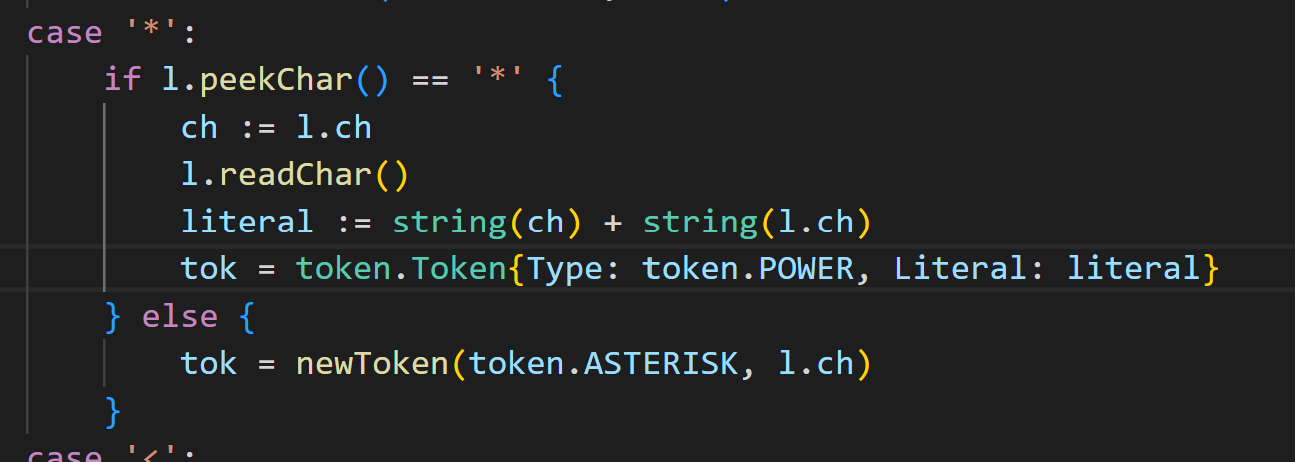
\includegraphics[width=0.5\linewidth]{images/2_lex.png}
    \label{fig:example}
\end{figure}
\begin{figure}[h]
    \centering
    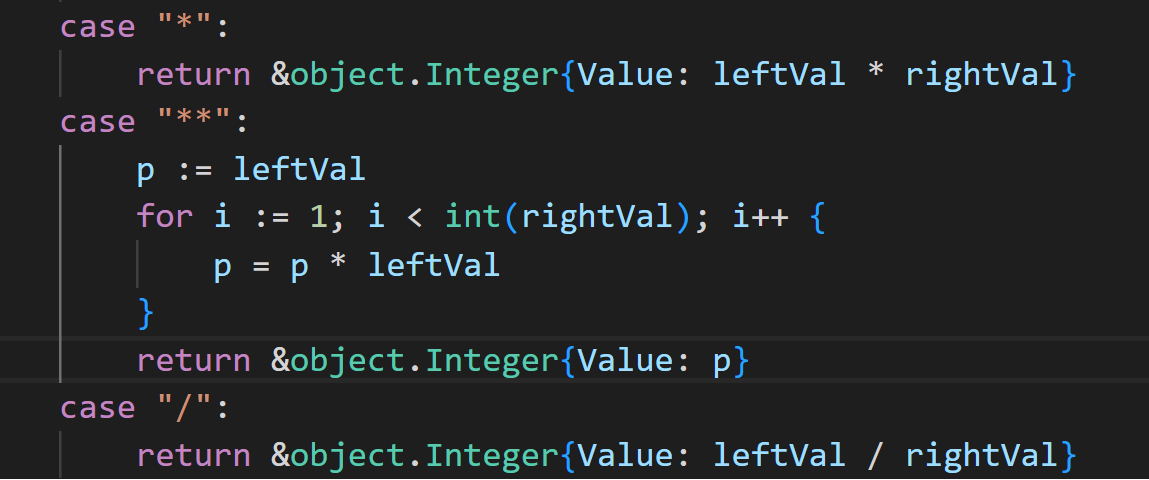
\includegraphics[width=0.5\linewidth]{images/2_eval.png}
    \label{fig:example}
\end{figure}

\begin{figure}[h]
    \centering
    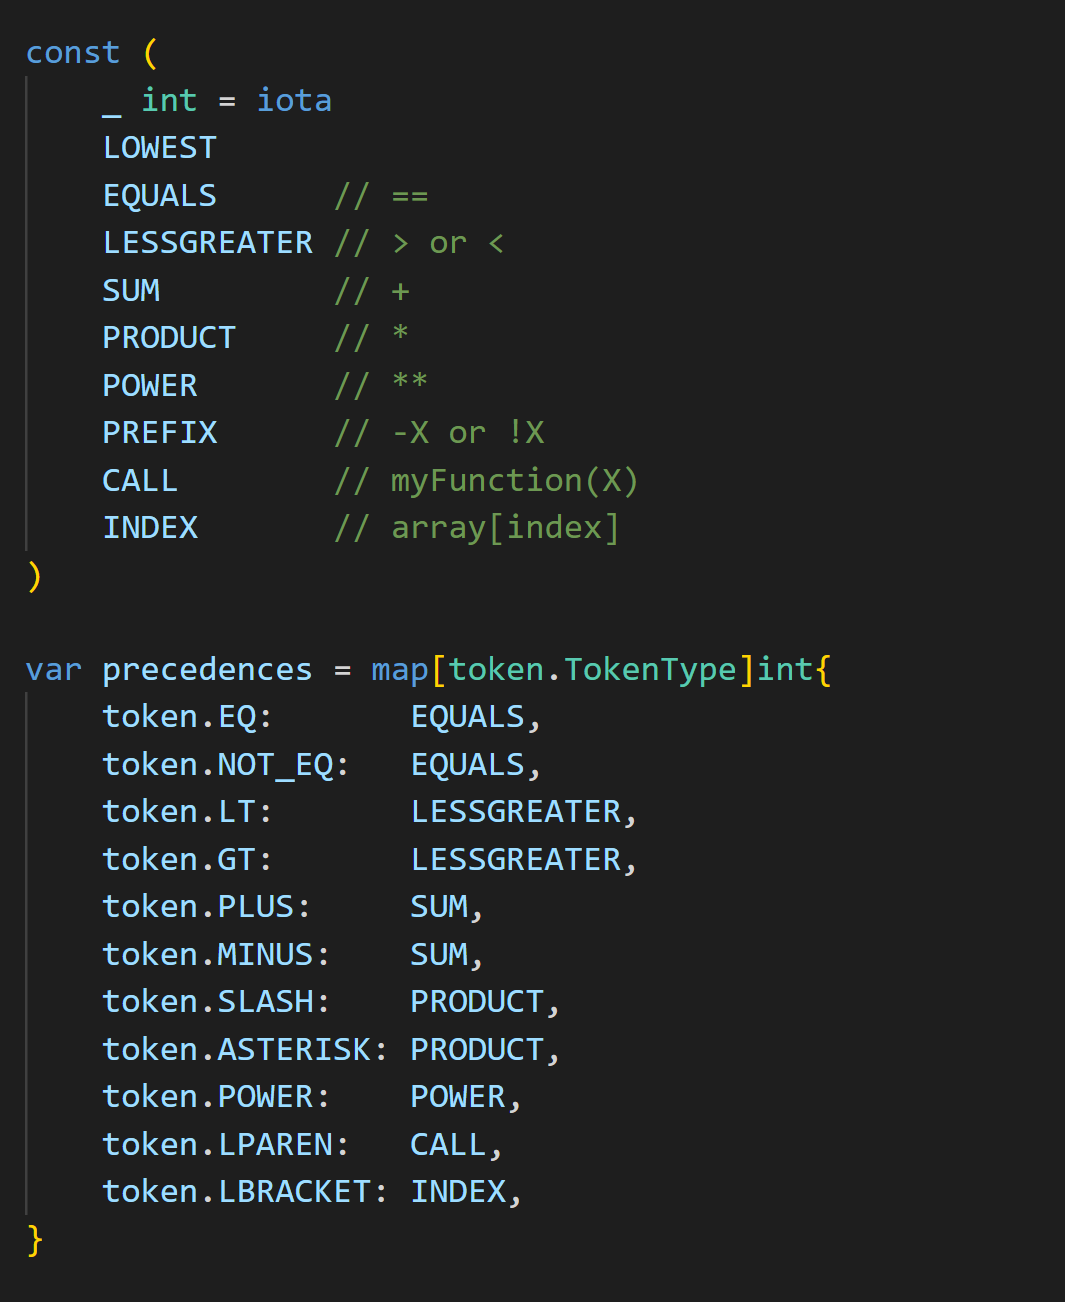
\includegraphics[width=0.5\linewidth]{images/2_par_1.png}
    \label{fig:example}
\end{figure}

\begin{figure}[h]
    \centering
    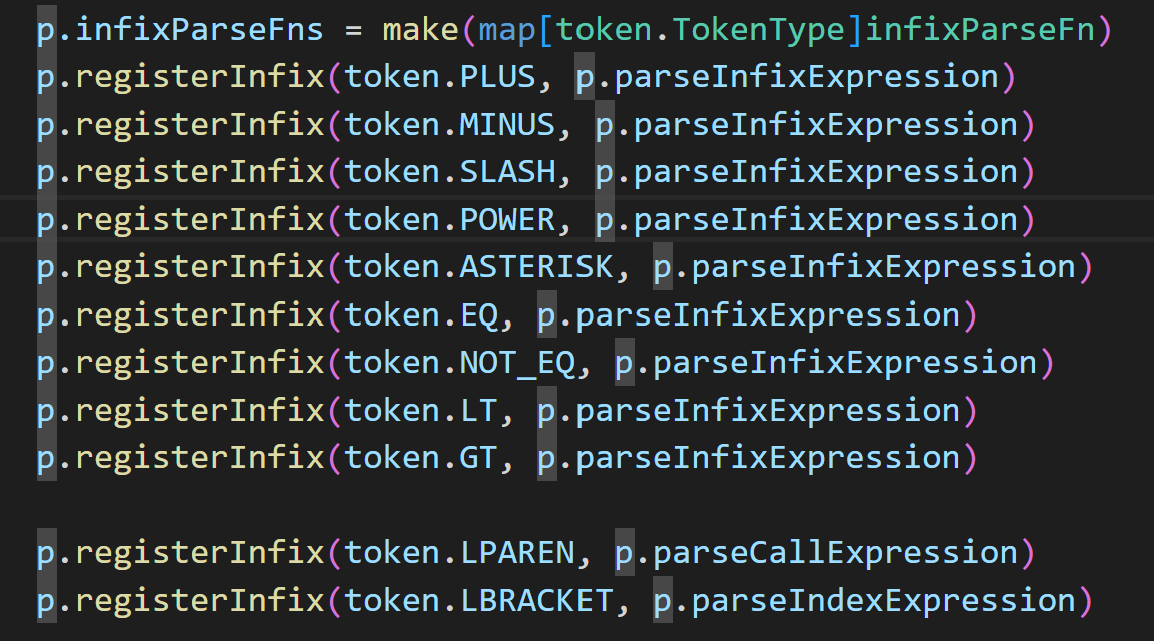
\includegraphics[width=0.5\linewidth]{images/2_par_2.png}
    \label{fig:example}
\end{figure}

\subsection{右結合}
べき乗を右結合とするためにはプログラムのどの部分を変更する必要がある
か.

parseInfixExpression関数で、べき乗演算子の右側にある式を再帰的に構文解析をするようにすることで、右結合になるはず.
また、evaluator内の evalInfixExpression 関数で、べき乗演算子の右結合を考慮して評価する必要がある.
\end{document}